\documentclass[12pt]{article}
\usepackage{graphicx}
\usepackage{amssymb}
\usepackage{epstopdf}
\usepackage{amsmath}
\usepackage{multicol}
\usepackage{tcolorbox}
\usepackage{geometry}
\usepackage{enumitem}
\usepackage{fancyhdr}

\DeclareGraphicsRule{.tif}{png}{.png}{`convert #1 `dirname #1`/`basename #1 .tif`.png}

\textwidth = 6.5 in
\textheight = 9 in
\oddsidemargin = 0.0 in
\evensidemargin = 0.0 in
\topmargin = -23pt
\headheight = 0.0 in
\headsep = 0.0 in
\parskip = 0.2in
\parindent = 0.0in
\pagestyle{fancy}
\pagenumbering{gobble}

\newtheorem{theorem}{Theorem}
\newtheorem{corollary}[theorem]{Corollary}
\newtheorem{definition}{Definition}
%\includegraphics [height=50mm, width=50mm]{PathInt.jpg}
\title{Title} 

\begin{document}
%INSTRUCTOR NOTES
%This activity aligns with a Desmos activity for exploring families of functions.

 Name:
 \begin{center}\large{4.3 Optimization Part 2}\end{center}

\begin{enumerate}

\item A manufacturer needs to make a cylindrical can that will hold 1.5 liters of liquid. Determine the dimensions of the can that will minimize the amount of material used in its construction. Note that $1$ Liter = $1000$ cm$^3$ and so we can convert $1.5$ liters into $1500$ cm$^3$.  The volume of a cylinder is $V = \pi r^2 h$ and surface area of cylinder is $A = 2\pi r h + 2\pi r^2$ (see digaram below).

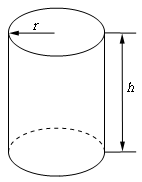
\includegraphics [scale=.7]{cyylinder-paulnotes.png}
\vfill

\item On the same side of a straight river are two towns, and both towns want to build a pumping station S. Where should the pumping station be located to minimize the TOTAL length of pipe used to connect each town to the pumping station?

\includegraphics [scale=.7]{4_3_pump}
\vfill

\newpage

$\hspace{10px}$ \\

\item A rectangle as one vertex on the origin and the other on the curve $y=e^{-2x}$. Estimate the maximum area of the rectangle.
\vfill

\item The product of two nonnegative numbers is 144. What is the minimum value of their sum?
\vfill

\end{enumerate}
\end{document}
%%%%%%%%%%%%%%%%%%%%%%%%%%%%%%%%%%%%%%%%%%%
